\documentclass[12pt]{article}
\textwidth 17cm \oddsidemargin 0cm \topmargin -2cm \textheight
24cm \footskip 1.5cm \usepackage{epsfig}
\usepackage{amsmath,graphicx,psfrag,pstcol,float,listings,color}
\usepackage{algorithm,algpseudocode,booktabs}
\usepackage{multirow}
\graphicspath{{./defn_files/}}
\def\n{\noindent}
\def\u{\underline}
\def\hs{\hspace}
\newcommand{\thrfor}{.^{\displaystyle .} .}
\newcommand{\bvec}[1]{{\bf #1}}

\usepackage{listings}
\usepackage{pdfpages}
\usepackage{fancyvrb}

\definecolor{mGreen}{rgb}{0,0.6,0}
\definecolor{mGray}{rgb}{0.5,0.5,0.5}
\definecolor{mPurple}{rgb}{0.58,0,0.82}
\definecolor{backgroundColour}{rgb}{0.95,0.95,0.92}

\lstdefinestyle{Matlab}{
    backgroundcolor=\color{backgroundColour},   
    commentstyle=\color{mGreen},
    keywordstyle=\color{magenta},
    numberstyle=\tiny\color{mGray},
    stringstyle=\color{mPurple},
    basicstyle=\footnotesize,
    breakatwhitespace=false,         
    breaklines=true,                 
    captionpos=b,                    
    keepspaces=true,                 
    numbers=left,                    
    numbersep=5pt,                  
    showspaces=false,                
    showstringspaces=false,
    showtabs=false,                  
    tabsize=2,
    language=Matlab
}

\begin{document}

\vspace{0.3cm}
\rule{15.7cm}{0.5mm}

\begin{center}
{\hspace{0.6cm}\Large \textbf {Software First Interim Report}\\
}
\end{center}
\begin{table}[H]
\centering
\begin{tabular}{ p{2cm}p{3cm}p{4cm} p{3cm}} 
&Brian Sun & Trinity College & gs534 \\ 
&Charles Zhou & Magdalene College & yz493 \\ 
&Paul Zhao & Magdalene College & yz496 \\ 
\end{tabular}
\end{table}


\begin{center}
\rule{15.7cm}{0.5mm}
\end{center}

\section{Introduction}
\n The aim of this project is to develop a logic simulation program in Python. Firstly teamwork planning is proposed. Then, the \textit{EBNF grammar} is defined, followed by the analyses of possible semantic errors based on the grammar, and relevant error handling approaches. Finally, two example logic definitions are given for demonstration. 
\section{Teamwork Planning}
\begin{table}[H]
\begin{tabular}{p{8cm}p{4cm}p{3cm}} 
\textit{Task names} & \textit{Assignee}&\textit{Duration}\\
\hline
Project outline and Task distribution & Brian Sun & 11/05 - 11/05\\
Version Control Setup & All members & 14/05 - 14/05\\
Grammar Draft 	& Charles Zhou & 12/05 - 13/05\\
Modification and Semantic Error & All members & 13/05 - 16/05\\
Description of Error Handling & Brian Sun & 16/05 - 17/05\\
Two examples & Paul Zhao & 16/05 - 17/05\\
Integration into a report & All members & 17/05 - 18/05\\
\end{tabular}
\caption{Week1 Language Definition and Project Plan}
\end{table}
\n The work in the first week focuses on the grammar definition and verification. After studying the EBNF together, Charles wrote the first draft of the \textit{Grammar}. Then, all three team members each came up with two circuit examples and wrote descriptions following the defined rules. In this process the grammar was checked, and semantic errors were listed. \\

\begin{table}[H]
\begin{tabular}{p{4.5cm}p{3.5cm}p{4cm}p{2.5cm}} 
\textit{Task names} & \textit{Assignee} & \textit{Code Reviewer} & \textit{Duration}\\
\hline
Names & Paul Zhao & Charles + Brian & 18/05 - 21/05\\
Scanner & Paul Zhao & Charles + Brian & 20/05 - 26/05\\
parse\_network & Paul Zhao & Charles + Brian & 23/05 - 27/05\\
top\_down\_parsing & Charlse Zhou & Paul + Brian & 20/05 - 27/05\\
error\_handling & Brian Sun & Paul + Charles & 25/05 - 28/05\\
Network Construction & Charles Zhou & Paul + Brian & 27/05 - 28/05\\
GUI Design & Brian Sun & Paul + Charlse & 18/05 - 28/05\\
Final Integration & All Members & N/A & 28/05 - 30/05\\
\end{tabular}
\caption{Week2\&3: Build and Test Individual Blocks}
\end{table}

\n Week 2 and 3 are the main period of constructing and testing the code. Tasks were assigned to each team member as in Table 2. The one who is assigned the task writes not only the module but also the \textit{pytest} where applicable. Though the task taker will be responsible to the module he writes, the reviewers need to review, comment and potentially modify the code, in order to ensure the quality and maintainability of the code. \par
\vspace{0.3cm}

\n According to the above task distribution, each team member is in charge of a big block, and this is also convenient for code maintenance. Once the change is announced, each member will quickly find the changes need to be done in his block, and do the necessary modifications. The allocation of responsibilities is listed below: 
\begin{table}[H]
\begin{tabular}{p{3cm}p{4cm}p{8cm}} 
Charles Zhou & in charge of & Grammar Definition and Top-down Parsing\\
Paul Zhao & in charge of & Scanner module and All interconnections\\
Brian Sun & in charge of & Error display and GUI\\
\end{tabular}
\caption{Week4: Maintenance}
\end{table}
\section{EBNF}

\section{Possible Semantic Errors}
\section{Error Handling}
\section{Examples of Definition Files}

\subsection{Sequential Carry Adder}
\begin{figure}[H]
    \centering
    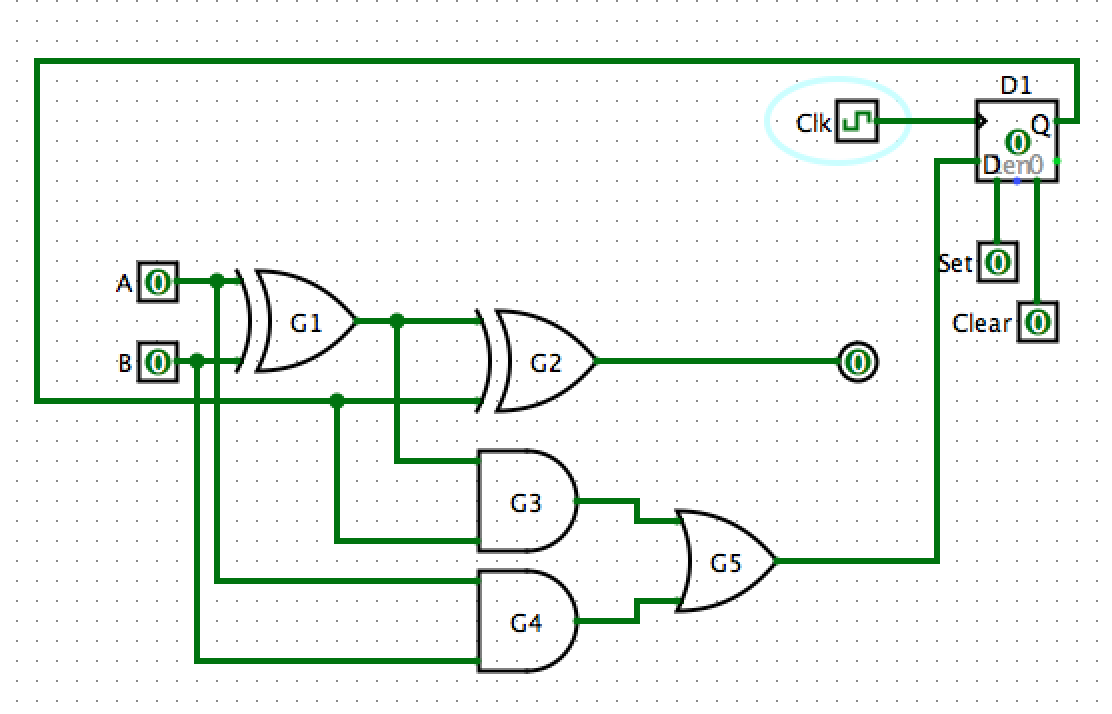
\includegraphics[scale=0.6]{sequential_carry_adder.png}
    \caption{circuit of a sequential carry adder}
\end{figure}



\subsection{Binary Multiplier}
\begin{figure}[H]
    \centering
    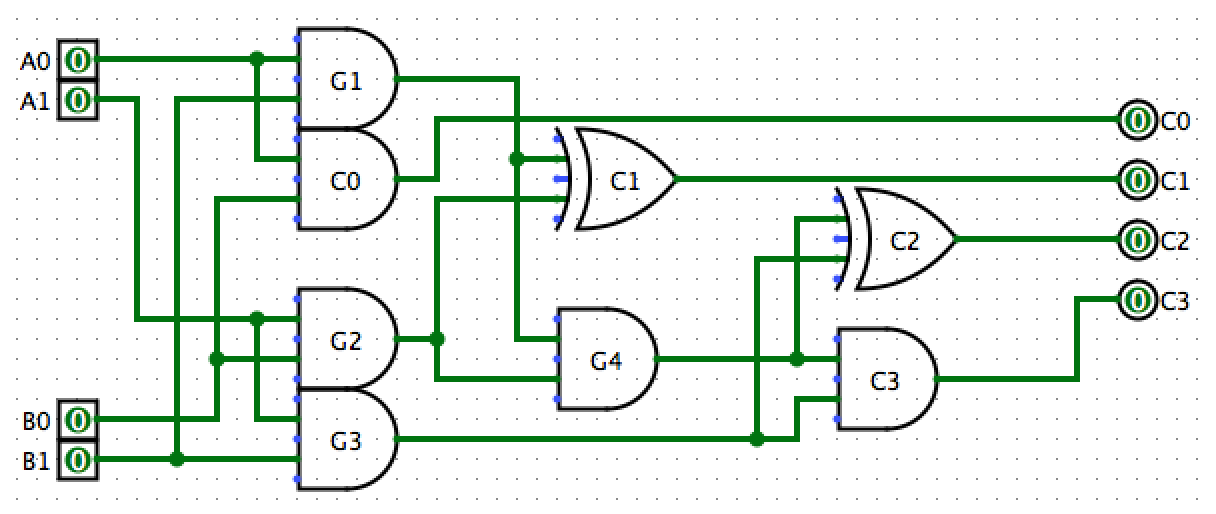
\includegraphics[scale=0.6]{bin_multiplier.png}
    \caption{circuit of a binary multiplier}
\end{figure}





\end{document}



\end{document}